\documentclass{standalone}
\usepackage{tikz}
\usetikzlibrary{patterns, positioning}
\usepackage[sfdefault]{ClearSans} %% option 'sfdefault' activates Clear Sans as the default text font
\usepackage[T1]{fontenc}

\begin{document}
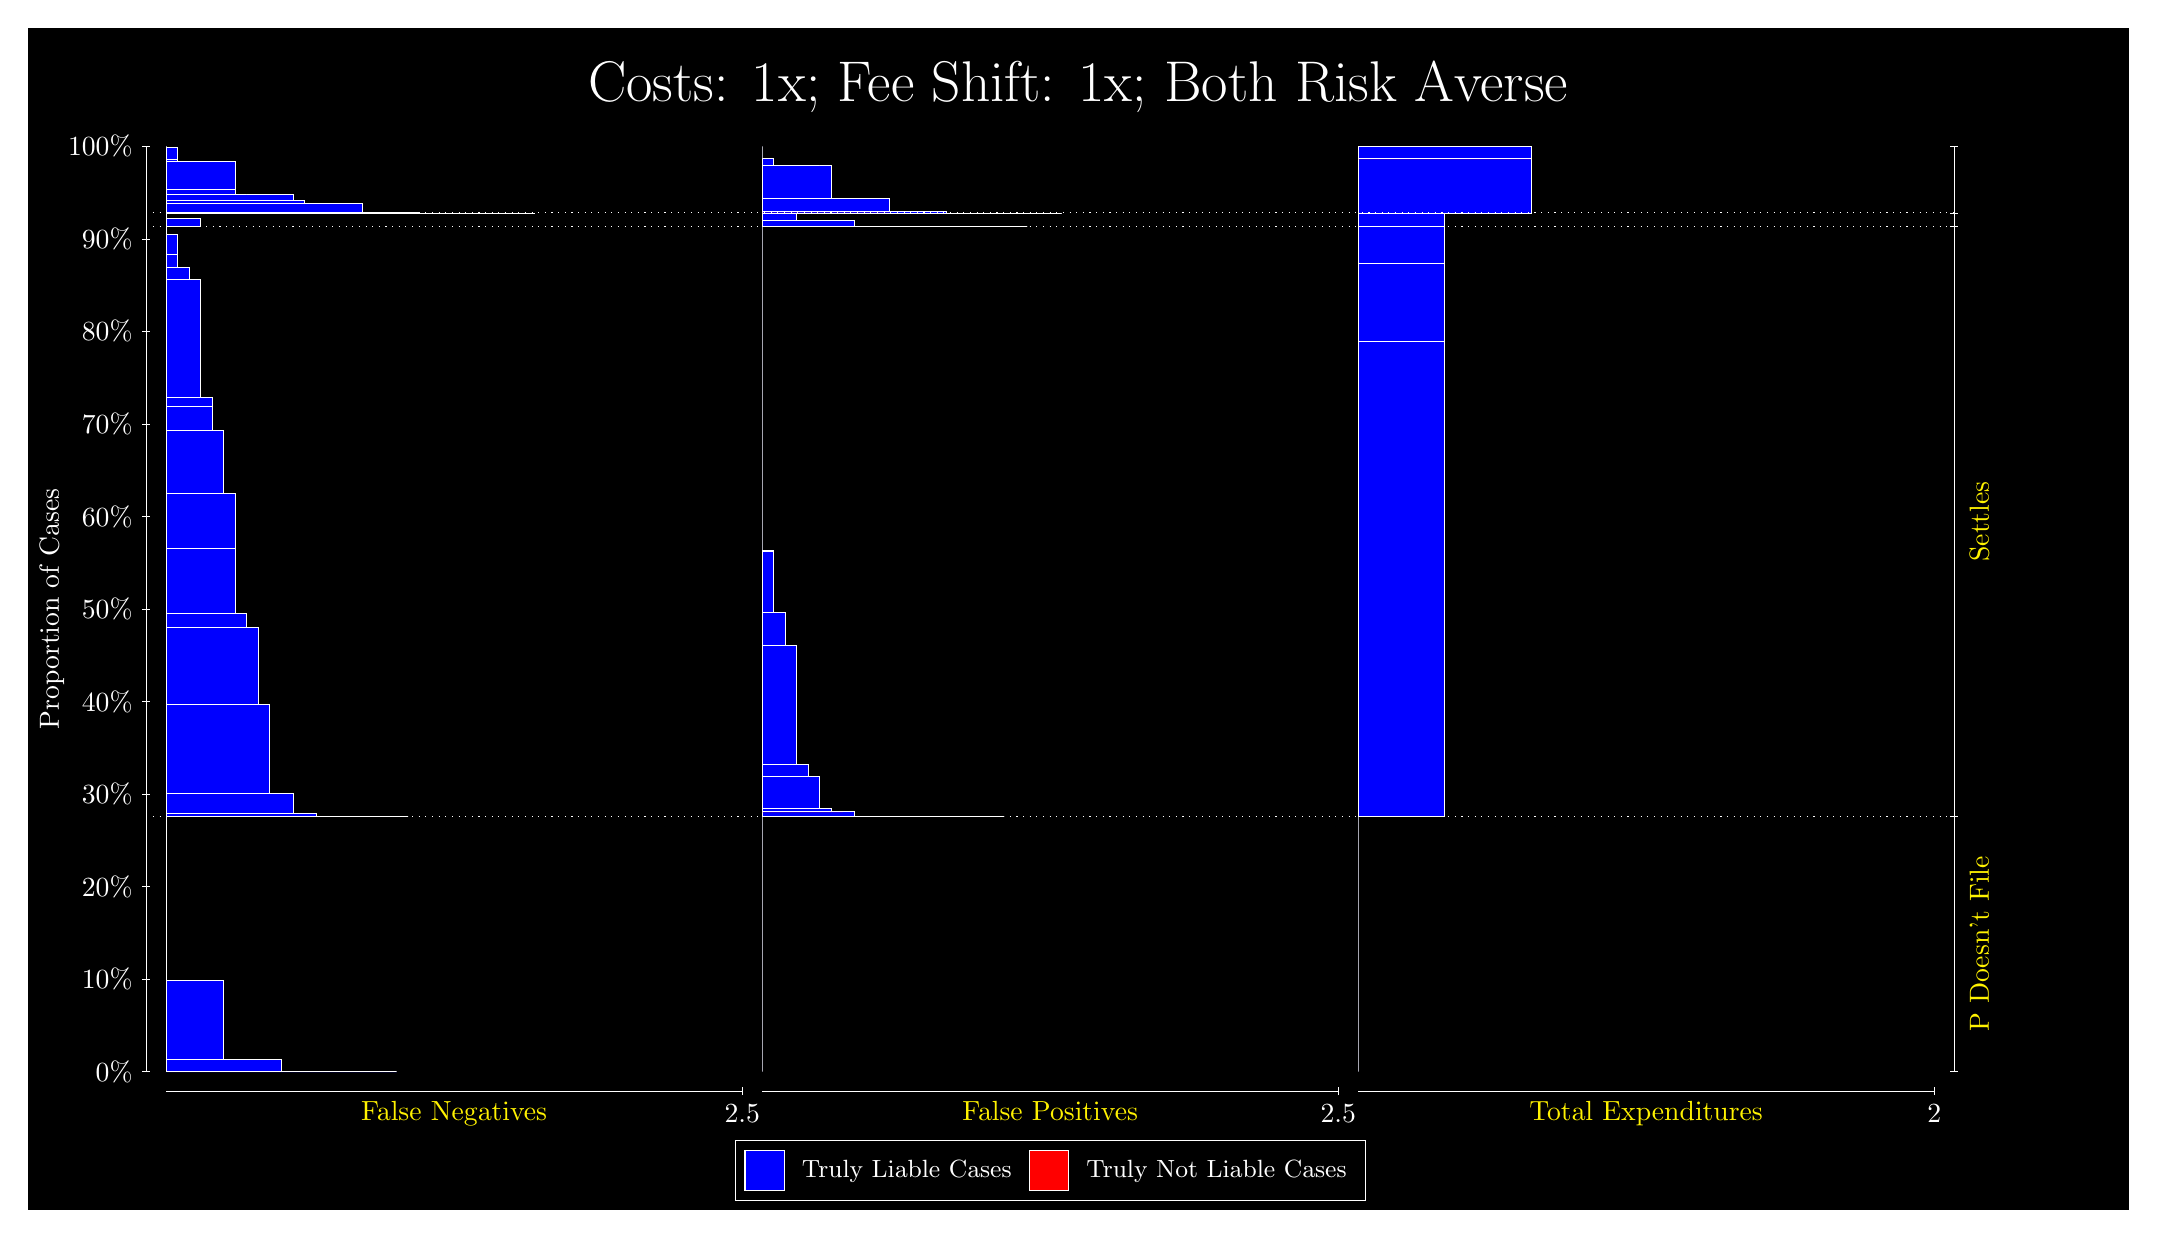
\begin{tikzpicture}
\draw[fill=black] (0,0) rectangle (26.667,15);
\draw[text=white] (0,13.5) rectangle (26.667,15) node[midway] {\huge Costs: 1x; Fee Shift: 1x; Both Risk Averse};
\draw[white, very thin] (1.5,1.75) -- (1.5,13.5);
\node[rotate=90, text=white, anchor=center] at (0.3, 7.625) {Proportion of Cases};
\draw[white, very thin] (1.45,1.75) -- (1.55,1.75);
\node[text=white, anchor=east] at (1.45, 1.75) {0\%};
\draw[white, very thin] (1.45,2.925) -- (1.55,2.925);
\node[text=white, anchor=east] at (1.45, 2.925) {10\%};
\draw[white, very thin] (1.45,4.1) -- (1.55,4.1);
\node[text=white, anchor=east] at (1.45, 4.1) {20\%};
\draw[white, very thin] (1.45,5.275) -- (1.55,5.275);
\node[text=white, anchor=east] at (1.45, 5.275) {30\%};
\draw[white, very thin] (1.45,6.45) -- (1.55,6.45);
\node[text=white, anchor=east] at (1.45, 6.45) {40\%};
\draw[white, very thin] (1.45,7.625) -- (1.55,7.625);
\node[text=white, anchor=east] at (1.45, 7.625) {50\%};
\draw[white, very thin] (1.45,8.8) -- (1.55,8.8);
\node[text=white, anchor=east] at (1.45, 8.8) {60\%};
\draw[white, very thin] (1.45,9.975) -- (1.55,9.975);
\node[text=white, anchor=east] at (1.45, 9.975) {70\%};
\draw[white, very thin] (1.45,11.15) -- (1.55,11.15);
\node[text=white, anchor=east] at (1.45, 11.15) {80\%};
\draw[white, very thin] (1.45,12.325) -- (1.55,12.325);
\node[text=white, anchor=east] at (1.45, 12.325) {90\%};
\draw[white, very thin] (1.45,13.5) -- (1.55,13.5);
\node[text=white, anchor=east] at (1.45, 13.5) {100\%};

\draw[white, very thin] (24.457,1.75) -- (24.457,13.5);
\draw[white, very thin] (24.407,1.75) -- (24.507,1.75);
\node[anchor=west] at (24.407, 1.75) {};
\draw[white, very thin] (24.407,4.9908) -- (24.507,4.9908);
\node[anchor=west] at (24.407, 4.9908) {};
\draw[white, very thin] (24.407,12.483) -- (24.507,12.483);
\node[anchor=west] at (24.407, 12.483) {};
\draw[white, very thin] (24.407,12.654) -- (24.507,12.654);
\node[anchor=west] at (24.407, 12.654) {};
\draw[white, very thin] (24.407,13.5) -- (24.507,13.5);
\node[anchor=west] at (24.407, 13.5) {};

\draw[white, very thin, fill=blue] (1.75,1.75) rectangle (4.6775,1.75);
\draw[white, very thin, fill=blue] (1.75,1.75) rectangle (3.9457,1.7513);
\draw[white, very thin, fill=blue] (1.75,1.7513) rectangle (3.2138,1.9013);
\draw[white, very thin, fill=blue] (1.75,1.9013) rectangle (2.4819,2.9095);
\draw[white, very thin, fill=red] (1.75,2.9095) rectangle (1.75,2.9095);
\draw[white, very thin, fill=blue] (1.75,2.9095) rectangle (1.75,4.9908);
\draw[white, very thin, fill=blue] (1.75,4.9908) rectangle (4.8239,4.9908);
\draw[white, very thin, fill=blue] (1.75,4.9908) rectangle (4.5312,4.9908);
\draw[white, very thin, fill=blue] (1.75,4.9908) rectangle (4.2384,4.9908);
\draw[white, very thin, fill=blue] (1.75,4.9908) rectangle (4.092,4.9908);
\draw[white, very thin, fill=blue] (1.75,4.9908) rectangle (3.9457,4.9908);
\draw[white, very thin, fill=blue] (1.75,4.9908) rectangle (3.7993,4.9908);
\draw[white, very thin, fill=blue] (1.75,4.9908) rectangle (3.6529,5.0323);
\draw[white, very thin, fill=blue] (1.75,5.0323) rectangle (3.5065,5.0332);
\draw[white, very thin, fill=blue] (1.75,5.0332) rectangle (3.3602,5.2838);
\draw[white, very thin, fill=blue] (1.75,5.2838) rectangle (3.2138,5.2846);
\draw[white, very thin, fill=blue] (1.75,5.2846) rectangle (3.0674,6.4134);
\draw[white, very thin, fill=blue] (1.75,6.4134) rectangle (3.0674,6.4194);
\draw[white, very thin, fill=blue] (1.75,6.4194) rectangle (2.921,7.3957);
\draw[white, very thin, fill=blue] (1.75,7.3957) rectangle (2.7746,7.5654);
\draw[white, very thin, fill=blue] (1.75,7.5654) rectangle (2.6283,8.3967);
\draw[white, very thin, fill=blue] (1.75,8.3967) rectangle (2.6283,9.0985);
\draw[white, very thin, fill=blue] (1.75,9.0985) rectangle (2.4819,9.8926);
\draw[white, very thin, fill=blue] (1.75,9.8926) rectangle (2.3355,10.202);
\draw[white, very thin, fill=blue] (1.75,10.202) rectangle (2.3355,10.315);
\draw[white, very thin, fill=blue] (1.75,10.315) rectangle (2.1891,11.815);
\draw[white, very thin, fill=blue] (1.75,11.815) rectangle (2.0428,11.969);
\draw[white, very thin, fill=blue] (1.75,11.969) rectangle (1.8964,12.125);
\draw[white, very thin, fill=blue] (1.75,12.125) rectangle (1.8964,12.381);
\draw[white, very thin, fill=blue] (1.75,12.381) rectangle (1.75,12.382);
\draw[white, very thin, fill=red] (1.75,12.382) rectangle (1.75,12.382);
\draw[white, very thin, fill=blue] (1.75,12.382) rectangle (1.75,12.483);
\draw[white, very thin, fill=blue] (1.75,12.483) rectangle (2.1891,12.58);
\draw[white, very thin, fill=red] (1.75,12.58) rectangle (1.75,12.58);
\draw[white, very thin, fill=blue] (1.75,12.58) rectangle (1.75,12.654);
\draw[white, very thin, fill=blue] (1.75,12.654) rectangle (6.4341,12.654);
\draw[white, very thin, fill=blue] (1.75,12.654) rectangle (5.7022,12.654);
\draw[white, very thin, fill=blue] (1.75,12.654) rectangle (4.9703,12.667);
\draw[white, very thin, fill=blue] (1.75,12.667) rectangle (4.8239,12.667);
\draw[white, very thin, fill=blue] (1.75,12.667) rectangle (4.2384,12.783);
\draw[white, very thin, fill=blue] (1.75,12.783) rectangle (4.092,12.783);
\draw[white, very thin, fill=blue] (1.75,12.783) rectangle (3.5065,12.809);
\draw[white, very thin, fill=blue] (1.75,12.809) rectangle (3.3602,12.896);
\draw[white, very thin, fill=blue] (1.75,12.896) rectangle (2.7746,12.896);
\draw[white, very thin, fill=blue] (1.75,12.896) rectangle (2.6283,12.952);
\draw[white, very thin, fill=blue] (1.75,12.952) rectangle (2.6283,13.308);
\draw[white, very thin, fill=blue] (1.75,13.308) rectangle (2.0428,13.308);
\draw[white, very thin, fill=blue] (1.75,13.308) rectangle (1.8964,13.337);
\draw[white, very thin, fill=blue] (1.75,13.337) rectangle (1.8964,13.485);
\draw[white, very thin, fill=red] (1.75,13.485) rectangle (1.75,13.485);
\draw[white, very thin, fill=blue] (1.75,13.485) rectangle (1.75,13.5);
\draw[white, very thin, fill=red] (9.3189,1.75) rectangle (9.3189,1.75);
\draw[white, very thin, fill=blue] (9.3189,1.75) rectangle (9.3189,4.9908);
\draw[white, very thin, fill=red] (9.3189,4.9908) rectangle (12.393,4.9908);
\draw[white, very thin, fill=blue] (9.3189,4.9908) rectangle (12.393,4.9908);
\draw[white, very thin, fill=red] (9.3189,4.9908) rectangle (11.807,4.9908);
\draw[white, very thin, fill=blue] (9.3189,4.9908) rectangle (11.807,4.9908);
\draw[white, very thin, fill=blue] (9.3189,4.9908) rectangle (11.661,4.9908);
\draw[white, very thin, fill=red] (9.3189,4.9908) rectangle (11.515,4.9908);
\draw[white, very thin, fill=blue] (9.3189,4.9908) rectangle (11.515,4.9908);
\draw[white, very thin, fill=red] (9.3189,4.9908) rectangle (11.222,4.9908);
\draw[white, very thin, fill=blue] (9.3189,4.9908) rectangle (11.222,4.9908);
\draw[white, very thin, fill=blue] (9.3189,4.9908) rectangle (11.075,4.9908);
\draw[white, very thin, fill=blue] (9.3189,4.9908) rectangle (10.929,4.9908);
\draw[white, very thin, fill=red] (9.3189,4.9908) rectangle (10.929,4.9908);
\draw[white, very thin, fill=blue] (9.3189,4.9908) rectangle (10.929,4.9908);
\draw[white, very thin, fill=blue] (9.3189,4.9908) rectangle (10.783,4.9911);
\draw[white, very thin, fill=red] (9.3189,4.9911) rectangle (10.636,4.9911);
\draw[white, very thin, fill=blue] (9.3189,4.9911) rectangle (10.636,4.9915);
\draw[white, very thin, fill=blue] (9.3189,4.9915) rectangle (10.49,5.0505);
\draw[white, very thin, fill=red] (9.3189,5.0505) rectangle (10.344,5.0505);
\draw[white, very thin, fill=blue] (9.3189,5.0505) rectangle (10.344,5.0606);
\draw[white, very thin, fill=blue] (9.3189,5.0606) rectangle (10.197,5.0918);
\draw[white, very thin, fill=blue] (9.3189,5.0918) rectangle (10.197,5.0924);
\draw[white, very thin, fill=red] (9.3189,5.0924) rectangle (10.051,5.0924);
\draw[white, very thin, fill=blue] (9.3189,5.0924) rectangle (10.051,5.505);
\draw[white, very thin, fill=blue] (9.3189,5.505) rectangle (9.9044,5.6582);
\draw[white, very thin, fill=blue] (9.3189,5.6582) rectangle (9.758,7.1588);
\draw[white, very thin, fill=blue] (9.3189,7.1588) rectangle (9.6116,7.581);
\draw[white, very thin, fill=blue] (9.3189,7.581) rectangle (9.4652,8.3574);
\draw[white, very thin, fill=blue] (9.3189,8.3574) rectangle (9.4652,8.3751);
\draw[white, very thin, fill=blue] (9.3189,8.3751) rectangle (9.3189,12.483);
\draw[white, very thin, fill=red] (9.3189,12.483) rectangle (12.686,12.483);
\draw[white, very thin, fill=blue] (9.3189,12.483) rectangle (12.686,12.483);
\draw[white, very thin, fill=blue] (9.3189,12.483) rectangle (11.954,12.483);
\draw[white, very thin, fill=blue] (9.3189,12.483) rectangle (11.222,12.483);
\draw[white, very thin, fill=blue] (9.3189,12.483) rectangle (10.49,12.557);
\draw[white, very thin, fill=blue] (9.3189,12.557) rectangle (9.758,12.654);
\draw[white, very thin, fill=red] (9.3189,12.654) rectangle (13.125,12.654);
\draw[white, very thin, fill=blue] (9.3189,12.654) rectangle (13.125,12.654);
\draw[white, very thin, fill=red] (9.3189,12.654) rectangle (12.393,12.654);
\draw[white, very thin, fill=blue] (9.3189,12.654) rectangle (12.393,12.654);
\draw[white, very thin, fill=red] (9.3189,12.654) rectangle (11.661,12.654);
\draw[white, very thin, fill=blue] (9.3189,12.654) rectangle (11.661,12.669);
\draw[white, very thin, fill=red] (9.3189,12.669) rectangle (10.929,12.669);
\draw[white, very thin, fill=blue] (9.3189,12.669) rectangle (10.929,12.846);
\draw[white, very thin, fill=red] (9.3189,12.846) rectangle (10.783,12.846);
\draw[white, very thin, fill=blue] (9.3189,12.846) rectangle (10.783,12.846);
\draw[white, very thin, fill=blue] (9.3189,12.846) rectangle (10.197,13.258);
\draw[white, very thin, fill=red] (9.3189,13.258) rectangle (10.051,13.258);
\draw[white, very thin, fill=blue] (9.3189,13.258) rectangle (10.051,13.258);
\draw[white, very thin, fill=blue] (9.3189,13.258) rectangle (9.4652,13.345);
\draw[white, very thin, fill=red] (9.3189,13.345) rectangle (9.3189,13.345);
\draw[white, very thin, fill=blue] (9.3189,13.345) rectangle (9.3189,13.5);
\draw[white, very thin, fill=red] (16.888,1.75) rectangle (16.888,1.75);
\draw[white, very thin, fill=blue] (16.888,1.75) rectangle (16.888,4.9908);
\draw[white, very thin, fill=red] (16.888,4.9908) rectangle (17.986,4.9908);
\draw[white, very thin, fill=blue] (16.888,4.9908) rectangle (17.986,11.025);
\draw[white, very thin, fill=red] (16.888,11.025) rectangle (17.986,11.025);
\draw[white, very thin, fill=blue] (16.888,11.025) rectangle (17.986,12.012);
\draw[white, very thin, fill=red] (16.888,12.012) rectangle (17.986,12.012);
\draw[white, very thin, fill=blue] (16.888,12.012) rectangle (17.986,12.483);
\draw[white, very thin, fill=red] (16.888,12.483) rectangle (17.986,12.483);
\draw[white, very thin, fill=blue] (16.888,12.483) rectangle (17.986,12.654);
\draw[white, very thin, fill=red] (16.888,12.654) rectangle (19.083,12.654);
\draw[white, very thin, fill=blue] (16.888,12.654) rectangle (19.083,13.345);
\draw[white, very thin, fill=red] (16.888,13.345) rectangle (19.083,13.345);
\draw[white, very thin, fill=blue] (16.888,13.345) rectangle (19.083,13.5);
\draw[white, dotted] (1.5,4.9908) -- (24.457,4.9908);
\draw[white, dotted] (1.5,12.483) -- (24.457,12.483);
\draw[white, dotted] (1.5,12.654) -- (24.457,12.654);
\draw[white, very thin] (1.75,1.5) -- (9.0689,1.5);
\node[text=yellow, anchor=north] at (5.4094, 1.5) {False Negatives};
\draw[white, very thin] (9.0689,1.45) -- (9.0689,1.55);
\node[text=white, anchor=north] at (9.0689, 1.45) {2.5};

\draw[white, very thin] (9.3189,1.5) -- (16.638,1.5);
\node[text=yellow, anchor=north] at (12.978, 1.5) {False Positives};
\draw[white, very thin] (16.638,1.45) -- (16.638,1.55);
\node[text=white, anchor=north] at (16.638, 1.45) {2.5};

\draw[white, very thin] (16.888,1.5) -- (24.207,1.5);
\node[text=yellow, anchor=north] at (20.547, 1.5) {Total Expenditures};
\draw[white, very thin] (24.207,1.45) -- (24.207,1.55);
\node[text=white, anchor=north] at (24.207, 1.45) {2};

\node[text=yellow, centered, rotate=90] at (24.777, 3.3704) {P Doesn't File};
\node[text=yellow, centered, rotate=90] at (24.777, 8.7368) {Settles};



\draw (12.978300999999998,1.5) node[draw=none] (baseCoordinate) {};
\begin{scope}[align=center]
        \matrix[scale=0.5, draw=white, below=0.5cm of baseCoordinate, nodes={draw}, column sep=0.1cm]{
            \node[rectangle, draw, minimum width=0.5cm, minimum height=0.5cm, fill=blue] {}; &
            \node[draw=none, font=\small, text=white] (B) {Truly Liable Cases}; &
            \node[rectangle, draw, minimum width=0.5cm, minimum height=0.5cm, fill=red] {}; &
            \node[draw=none, font=\small, text=white] (B) {Truly Not Liable Cases}; \\
            };
\end{scope}

\end{tikzpicture}
\end{document}